\documentclass[twocolumn]{article}

\usepackage{geometry}
\geometry{a4paper, margin=1in}
\usepackage[utf8]{inputenc}
\usepackage[T1]{fontenc}
\usepackage{lmodern}
\usepackage[english]{babel}
\usepackage{hyperref}
\usepackage{graphicx}

\begin{document}
	\title{Deep learning homework project: \ Waste classification}
	\author{Anna Gergály, Péter Mészáros}
	\maketitle
	
	\section{Introduction}
	Lot of waste. Waste management on this scale poses a lot of challenges and risks, both economically and environmentally. One of the best solutions we know at the moment besides trying to reduce the amount of waste created is to recycle. This helps recover resources and decreases chance of pollution and mitigates energy usage. 
	
	Despite it's obvious benefits it is not practiced at a large enough extent. The reasons for this mainly stem from the same issue: the need to separate the different materials. At home recycling often fails due to the cumbersome nature of the activity and in-facility waste separation is a very difficult task: manual classification is almost impossible due to sheer quantity and automatic waste sorting usually only works for certain materials in certain conditions.
	
	Our goal in this project was to create and review different solutions for a deep learning system that could provide automatic waste classification in such an environment.
	\section{Previous solutions}\label{sec:prevsolutions}
	In \cite{Chu2018} a complex hardware-software solution with a multilayer hybrid method was proposed to classify waste into recyclable and non-recyclable classes and they achieved over 90\% mean accuracy. They cite previous solutions made with R-CNN, CNN and SVM classifiers with accuracy rates ranging from 23\% to 77\%. They trained the model with images of wastes found in urban public areas, in total of 22 classes.
	
	The CNN they used in \cite{Chu2018} was a modified version of AlexNet \cite{AlexNet} consisted of 5 convolution layers, 3 max-pooling layers and 3 dense layers in the end. The input image size was 240$\times$240, the convolution kernel sizes were 11$\times$11 for the first, 5$\times$5 for the second and 3$\times$3 for the last 3 convolutional layers. The first two dense layers had 512 neurons. The last dense layer had 22 neurons to match the number of classes. After this an additional layer was added during training with 1 neuron to classify into recyclable and non-recyclable.
	
	They achieved accuracy and recall over 90\% with only the CNN, but the metrics were even better when they added extra information by other sensor (e. g. weight).
	
	In \cite{ADEDEJI2019607} a pre-trained ResNet-50 \cite{DBLP:journals/corr/HeZRS15}
	network was used for recognition with a Support Vector Machine (SVM) classifier. The dataset is from \cite{yang2016classification} which turned out to be one of the datasets we used from Kaggle. (The dataset from Kaggle is just a subset of the original. \cite{cchangcs_2018}) They achieved 87\% accuracy after 12 epochs trained with SGDM optimizer.
	
	In \cite{10.1145/3417473.3417474} a pre-trained Inception-v3 was further trained to classify waste. The initial training was done on the ImageNet \cite{5206848} dataset. The training and testing was done using a Raspberry Pi 3B, exceptional results were achieved with 92.5\% with a similar training dataset to the previous one.
	
	\section{Dataset}
	We assembled our dataset from 3 online sources (2 from Kaggle and 1 from Github) both to have a larger pool of images and a more varied one. There are pictures that contain the discarded item in front of plain backgrounds and ones that show them in a more organic way: dirty and/or muddy on a floor. 
	
	We settled on having eight categories within the datasets. These (glass, paper, cardboard, trash, metal, plastic, e-waste, medical) were selected mainly on two grounds: the available data and practical considerations. Most of these are well-known, already used recycling categories (glass, paper, cardboard, metal, plastic) and we have a multiple classes for non-recyclables, too. The main one of these is trash, but having extra categories for e-waste and medical waste makes sense as these are more dangerous environmentally and public health-wise. To make our datasets conform to these categorical standards we rearranged some of the pre-labeled data: e.g. merged different colored glasses and deleted categories we deemed unnecessary.
	
	The datasets together hold about 23,000 images which we decided to split in 14:3:3 ratio into training, validation and test sets.\ref{dataset} On the training set we decided to employ data augmentation: using the keras ImageDatasetGenerator we added zooming and shifting as well as both vertical and horizontal flips and 90° rotation to account for the fact that these items could be seen in any orientation in a waste management scenario.
	
	\begin{figure}[htb]
		\centering
		\resizebox{\linewidth}{!}{
			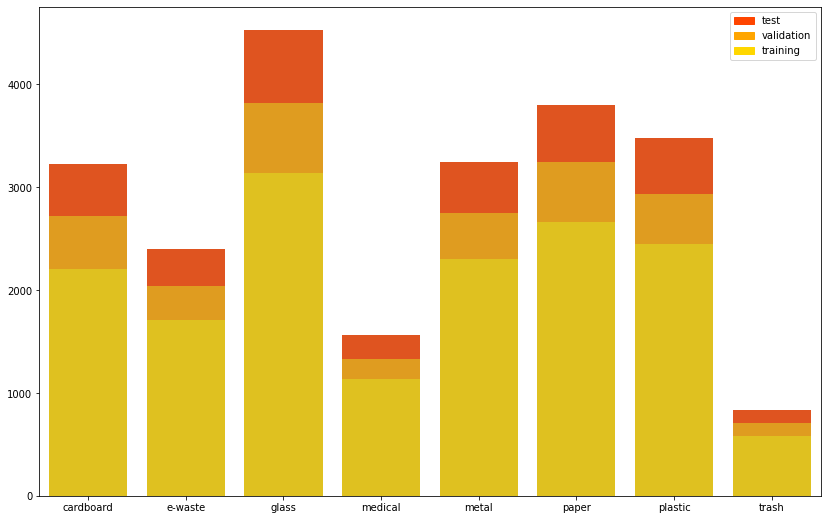
\includegraphics{dataset.png}}
		\caption{The size of the classes as divided into training, validation and test sets.}
		\label{dataset}
	\end{figure}
	
	\section{Proposed method}
	
	Our approach was to try out multiple pre-trained image classification CNNs by using transfer learning to prepare them for our specific task. The ones we use are EfficientNetB5 and MobileNetV2, both pre-trained on the imagenet dataset. To add a bit more interest and challenge to task we also decided to try our hands at building our own CNN from scratch.
	
	\subsection{EfficientNetB5}
	
	We chose the B5 variant of the EfficientNet because of it's moderate size and fairly strong results. We wanted something that would be feasible to train given our limited GPU-resources, but had a high-chance of yielding acceptable results. We removed the top-layer and substituted it with a few fit for our own needs: global average pooling, dropout and a dense layer with 8-nodes and a softmax activation to serve as an output layer in the 8-class classification problem.
	
	We trained this model, with only transfer learning using categorical crossentropy as our loss and categorical accuracy as our main metric, we used early stopping to stop the model from overfitting. The chosen batch size was 32, and 400 steps per epoch. We achieved a quite good result with this method (\textasciitilde$~87\% $ categorical accuracy) and we decided to go on with fine-tuning this model. 
	
	This however, was not possible, due to our technical limitations: the Google Colab environment could not support training this large of a model. This was one of the reasons we decided on a MobileNet for the third model: we wanted a transfer learning solution where we could also employ fine-tuning. 
	
	\subsection{Our own model}
	
	
	
	\subsection{MobileNetV2}
	
	
	
	\section{Evaluation method}
	For evaluating the trained models, we used a few metrics. The metrics were calculated using sklearn. The calculated metrics are accuracy, balanced accuracy, precision (weighted), recall (weighted), f1 score (weighted) and top2 and top3 accuracy. Of course the top2 and top3 accuracies are less important because of the small number of classes.
	
	\section{Results}
	The best results were achieved with the EfficientNetB5, the accuracy on the test dataset is 89.9\%. The accuracy achieved with MobileNetV2 was 83.5\%. On our own model the accuracy was about 50\%.
	
	\begin{figure}
		\centering
		\resizebox{\linewidth}{!}{
			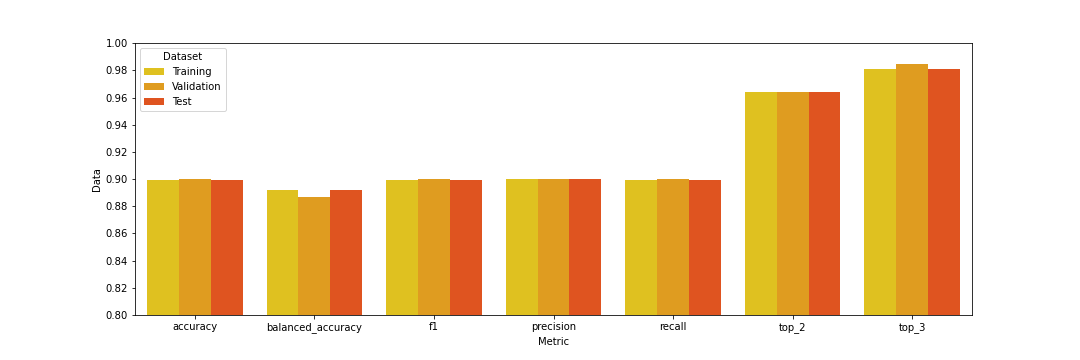
\includegraphics{model1_metrics.png}}
		\caption{The evaluated metrics on the first model.}
		\label{dataset}
	\end{figure}
	\begin{figure}
		\centering
		\resizebox{\linewidth}{!}{
			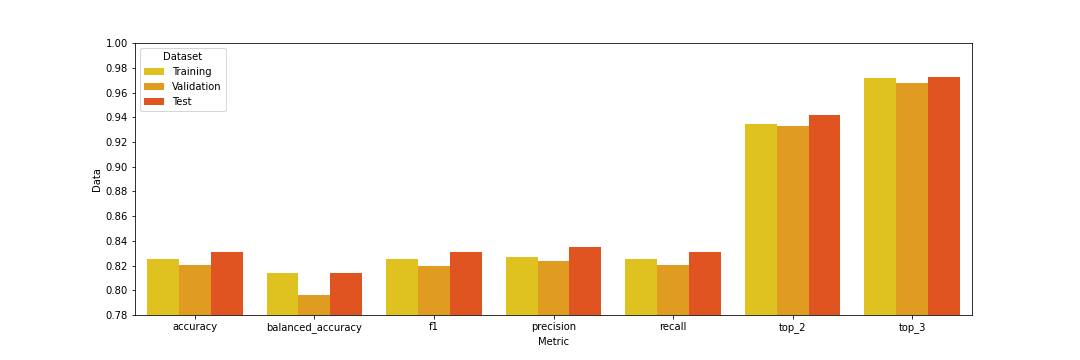
\includegraphics{model3_metrics.png}}
		\caption{The evaluated metrics on the third model.}
		\label{dataset}
	\end{figure}
	
	\section{Discussion}
	The results with the best models are comparable to the results which we've seen and covered in section \ref{sec:prevsolutions}.
	Our own model had the worse results, but they are still better than random chance. The main reason could be the small number of images compared to the ImageNet dataset which the other models were pre-trained on. The model complexity and size can also we a hurdle, but as we've seen in \cite{Chu2018}, great results can be achieved which smaller (in terms of layer number) models.
	The best results were achieved with the EfficientNetB5 which is not surprising because it's the largest model out of the three with about 30 million parameters. With the MobileNetV2 the accuracy was worse, but that model has about 3 million parameters and the inference time on a GPU is more than 6 times better (according to the Keras site \cite{keras_applications}).
	
	\bibliographystyle{unsrt}
	\bibliography{irodalom}
	
\end{document}